% Created 2022-05-24 di 23:53
% Intended LaTeX compiler: pdflatex
\documentclass[11pt]{article}
\usepackage[utf8]{inputenc}
\usepackage[T1]{fontenc}
\usepackage{graphicx}
\usepackage{grffile}
\usepackage{longtable}
\usepackage{wrapfig}
\usepackage{rotating}
\usepackage[normalem]{ulem}
\usepackage{amsmath}
\usepackage{textcomp}
\usepackage{amssymb}
\usepackage{capt-of}
\usepackage{hyperref}
\author{vimmoos}
\date{\today}
\title{Uncertainty in Machine Learning $\backslash$\ Assignment 1}
\hypersetup{
 pdfauthor={vimmoos},
 pdftitle={Uncertainty in Machine Learning $\backslash$\ Assignment 1},
 pdfkeywords={},
 pdfsubject={},
 pdfcreator={Emacs 26.3 (Org mode 9.1.9)},
 pdflang={English}}
\begin{document}

\maketitle
\tableofcontents


\section{Sources of Uncertainty}
\label{sec:org4e57f4d}
\subsection{Aleatoric}
\label{sec:org4d0b1e3}
\begin{itemize}
\item The first example of Aleatoric uncertainty can be when we are
dealing with robots and the input to the neural network is a sensor.
If the sensor is not perfect or is not correctly calibrated or even
worse has some technical problems, the data that we will gather will
be noisy/imperfect. This will be a case of aleatoric uncertainty
since the uncertainty is an intrinsic property of the data we get.

\item Another example of Aleatoric uncertainty can be when we train a
neural network (for classification) with blurred images. This is a
clear instance of Aleatoric uncertainty since the uncertainty comes
from the data itself and not from the model. Moreover, having more
training examples does not alleviate this type of uncertainty.
\end{itemize}

\subsection{Epistemic}
\label{sec:org97222da}
\begin{itemize}
\item A famous example of epistemic uncertainty, happened when some service
for facial recognition failed to recognize afro-american women. This
happened because of the lack of data. In particular, the problem was
that the data they used to train the network was biased on white men
and there were few or no data points for afro-american in
general. This is an example of epistemic uncertainty since given
more data the neural network would have been able to solve this
problem and correctly categorise every face.

\item Another example of epistemic uncertainty, can be when we train a
network on some data set, let's say MNIST (digits), and then we try
to categorise letters. This is a clear and simple example of
model misspecification.
\end{itemize}
\section{Are They Probabilities?}
\label{sec:org64fa31c}
\subsection{DUQ}
\label{sec:orgccf721a}
In the case of DUQ, the confidence outputs can be  considered
probabilities but not in the intuitive sense.
More specifically, DUQ uses a radial basis function (RBF) for measuring
uncertainty. The RBF measures the distance between the model output
and the centroids. Generally, RBFs are bounded between 0 and 1.
Which is in line with a probabilistic interpretation.
Another important point, in interpreting the confidence outputs of the
DUQ under a probabilistic framework is that the confidence outputs
are not probabilities but likelihoods.

Take a look at the formula of the RBF:

\begin{equation}
\label{eq:org91d67d6}
K_c(f_{\theta}(x),e_c) = exp\left(- \frac{\frac{1}{n} \| W_cf_{\theta}(x)
-e_c \|_2^2}{2\sigma^2}\right)
\end{equation}

we can notice that it is structurally similar to the probability
density function of an isotropic (rotationally invariant)
D-dimensional gaussian distribution:

\begin{equation}
\label{eq:orgee68179}
\mathcal{N}(x | \mu,\sigma^2I) = (2\pi\sigma^2)^{-\frac{D}{2}} exp
\left(- \frac {\| x - \mu \|^2} {2\sigma^2} \right)
\end{equation}

In light of this, we can say that the output of DUQ is proportional to the
probability density under an isotropic Gaussian.
Therefore, it is clear that the confidence outputs can be considered
as probabilities (to be strict we should say likelihoods and not probabilities)
\subsection{Gradient Uncertainty}
\label{sec:org92c31b1}
In the case of the Gradient Uncertainty, the confidence outputs cannot
be considered as probabilities.
In the paper, they stated: "We interpret this
're-learning-stress' as uncertainty". This 're-learning-stress' is
based on the gradient and therefore is highly coupled to the model and
its parameters. It is therefore impossible to interpret this type of
uncertainty as some kind of probability or likelihood.
\section{Programming}
\label{sec:orgbfcde54}
We have created a dataset based on the tanh function. We have added a
Gaussian noise with parameters \(\mu\) = 0 and \(\sigma\) = 0.5. The results
show that our neural network learned the function quite well as we
can see from the predicted mean. On the other hand, for the predicated
variance, we can see that the neural network correctly estimates the
aleatoric uncertainty. The mean of the predicted \(\sigma\) is 0.55891913
which is a slightly overestimate but it is quite good.
Below is the graph of the data points, predictions and actual function.
\begin{center}
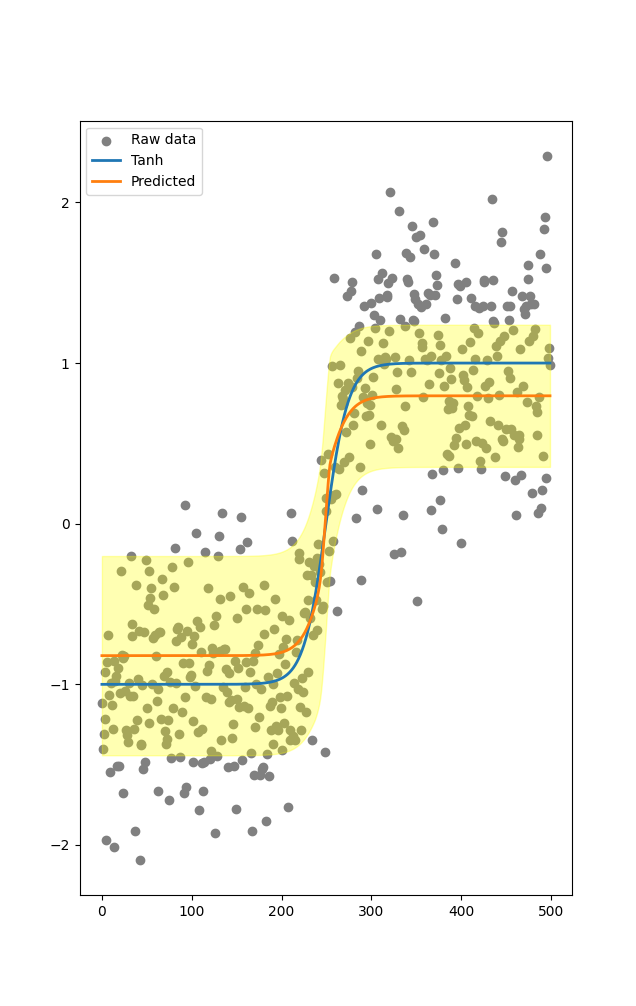
\includegraphics[width=.9\linewidth]{./tanh.png}
\end{center}
\end{document}
